\section{Relation to VED}
\label{sec:ved_relation}

\subsection{Division of roles}
\label{subsec:division_of_roles}

IFGT is not an independent foundational theory but an upper-layer effective theory that describes the \emph{unclosed side} of the generative structure described by Vortical Enclosure Dynamics (VED).

The division of roles between VED and IFGT is organized as follows.

\begin{itemize}
  \item \textbf{VED}: Describes the \emph{generation} of physical structure from difference, gradient, flow, and closure. It treats stable structures, particles, fields, and spacetime that are realized through the closure degree $C$.
  \item \textbf{IFGT}: Within the same generative structure, treats the informational structure that persists as a \emph{quasi-closure} in the region where $C$ does not reach unity.
\end{itemize}

VED addresses the side where closure succeeds; IFGT addresses the side where closure remains incomplete. The two are not opposing theories but complementary descriptions of the same generative structure viewed from different aspects. This division is visualized in Fig.~\ref{fig:two_aspects}.

\begin{figure}[h]
  \centering
  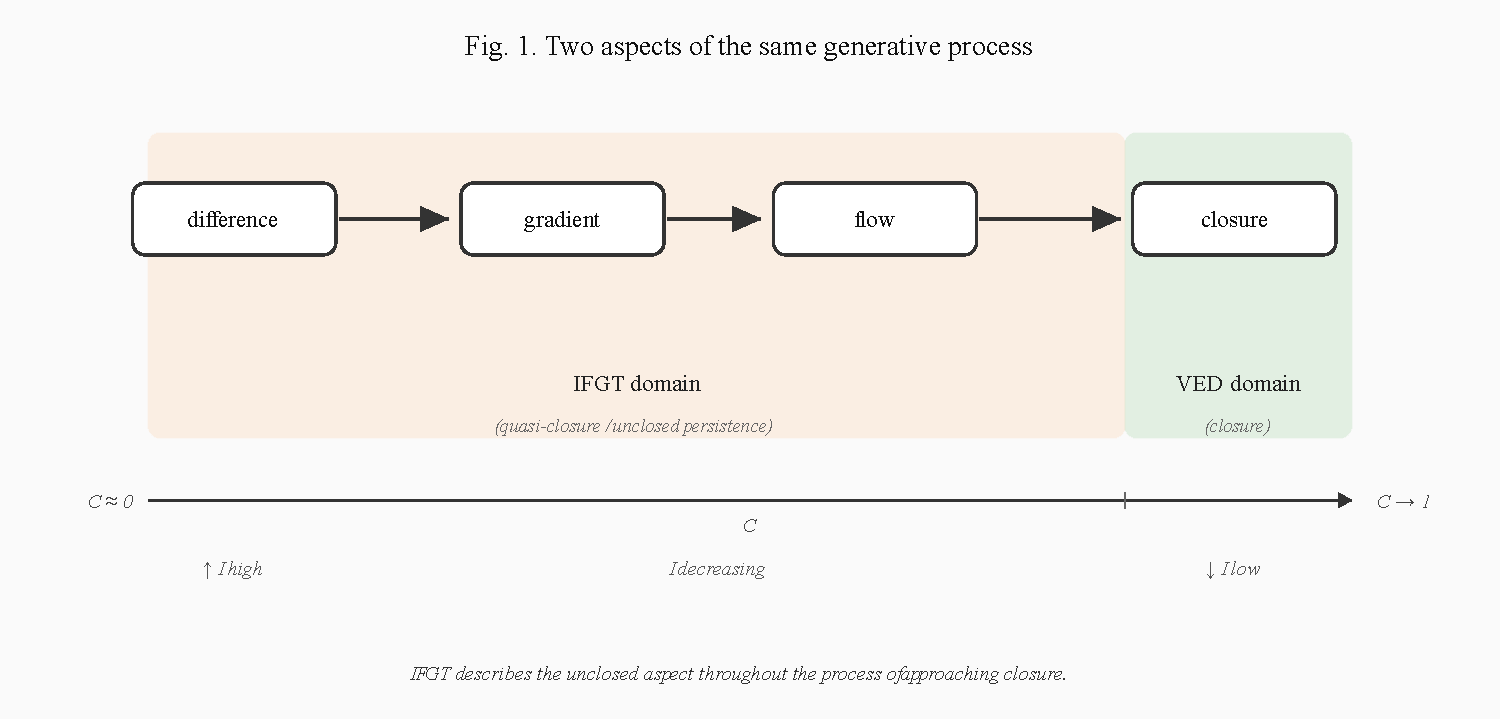
\includegraphics[width=0.95\textwidth]{figures/fig1_two_aspects_en.pdf}
  \caption{Two aspects of the same generative process. The VED chain (difference $\to$ gradient $\to$ flow $\to$ closure) unfolds across the closure-degree axis $C$. IFGT covers the region where $C$ has not yet reached unity; VED describes the fully closed region.}
  \label{fig:two_aspects}
\end{figure}

\subsection{The asymmetry between \texorpdfstring{$I$}{I} and \texorpdfstring{$C$}{C}}
\label{subsec:asymmetry}

The central quantity of VED is the closure degree $C \in [0, 1]$. The central quantity of IFGT, the information density $I$, is related to $C$ by
\begin{equation}
I = f(1 - C),
\label{eq:I-C-relation}
\end{equation}
where $f$ is a non-decreasing function satisfying $I \to 0$ as $C \to 1$. In the region of complete closure, where $C$ reaches unity, information does not exist; information is defined only in the region where $C < 1$.

This relation shows that $I$ and $C$ are \emph{not two expressions of the same quantity but complementary quantities}. $C$ describes ``the degree of closedness,'' while $I$ describes ``the density of the residue that failed to close.'' Both arise from the same field but can behave as independent quantities (for example, two regions with the same $C$ may have different spatial distributions of $I$ depending on their history).

This asymmetry is precisely what embodies the division of roles between VED and IFGT at the level of variables.

\subsection{Informational time \texorpdfstring{$\tau$}{tau} and generative time \texorpdfstring{$\tau_{\mathrm{VED}}$}{tau-VED}}
\label{subsec:time}

Three notions of time appear in this paper; we organize them here.

\begin{itemize}
  \item \textbf{Ordering parameter $t$}: an externally given time axis. It is meaningful only in the effective description where the background spacetime is fixed (see~§\ref{sec:unified_equation}).
  \item \textbf{Generative time $\tau_{\mathrm{VED}}$}: the observational time of VED Vol.~1. It is defined endogenously as the progression of difference consumption accompanying closure formation.
  \item \textbf{Informational time $\tau$}: the time introduced in IFGT. It is defined endogenously as the accumulation of \emph{mutual interference between difference and the existing trace structure}.
\end{itemize}

$\tau_{\mathrm{VED}}$ and $\tau$ \emph{differ in origin}. The former advances as closure proceeds; the latter advances as traces are updated.

Nevertheless, the two are \emph{dynamically isomorphic}. Both are not externally given parameters but quantities generated endogenously from the internal difference dynamics of the system, and both are irreversible. Accordingly, this theory treats IFGT's $\tau$ as a quantity embeddable on the same temporal axis as VED's $\tau_{\mathrm{VED}}$. It should be noted, however, that the two quantities measure different aspects of the same phenomenon and cannot be fully identified.

\subsection{The circular relation}
\label{subsec:circular}

The relation between VED and IFGT is not a unidirectional reduction. The informational quasi-closure is not merely added on top of physical structure; through its mutual interference with physical structure, it alters subsequent difference generation and flow. Conversely, physical structure produces new differences, which in turn form informational structures as quasi-closures.

\begin{equation}
\text{difference}
\xrightarrow{\text{partial closure}}
\text{quasi-closure (IFGT)}
\xrightarrow{\text{constraint}}
\text{structure (VED)}
\xrightarrow{\text{regeneration}}
\text{difference}
\label{eq:cycle}
\end{equation}

This cyclic relation is depicted in Fig.~\ref{fig:cyclic_relation}.

\begin{figure}[h]
  \centering
  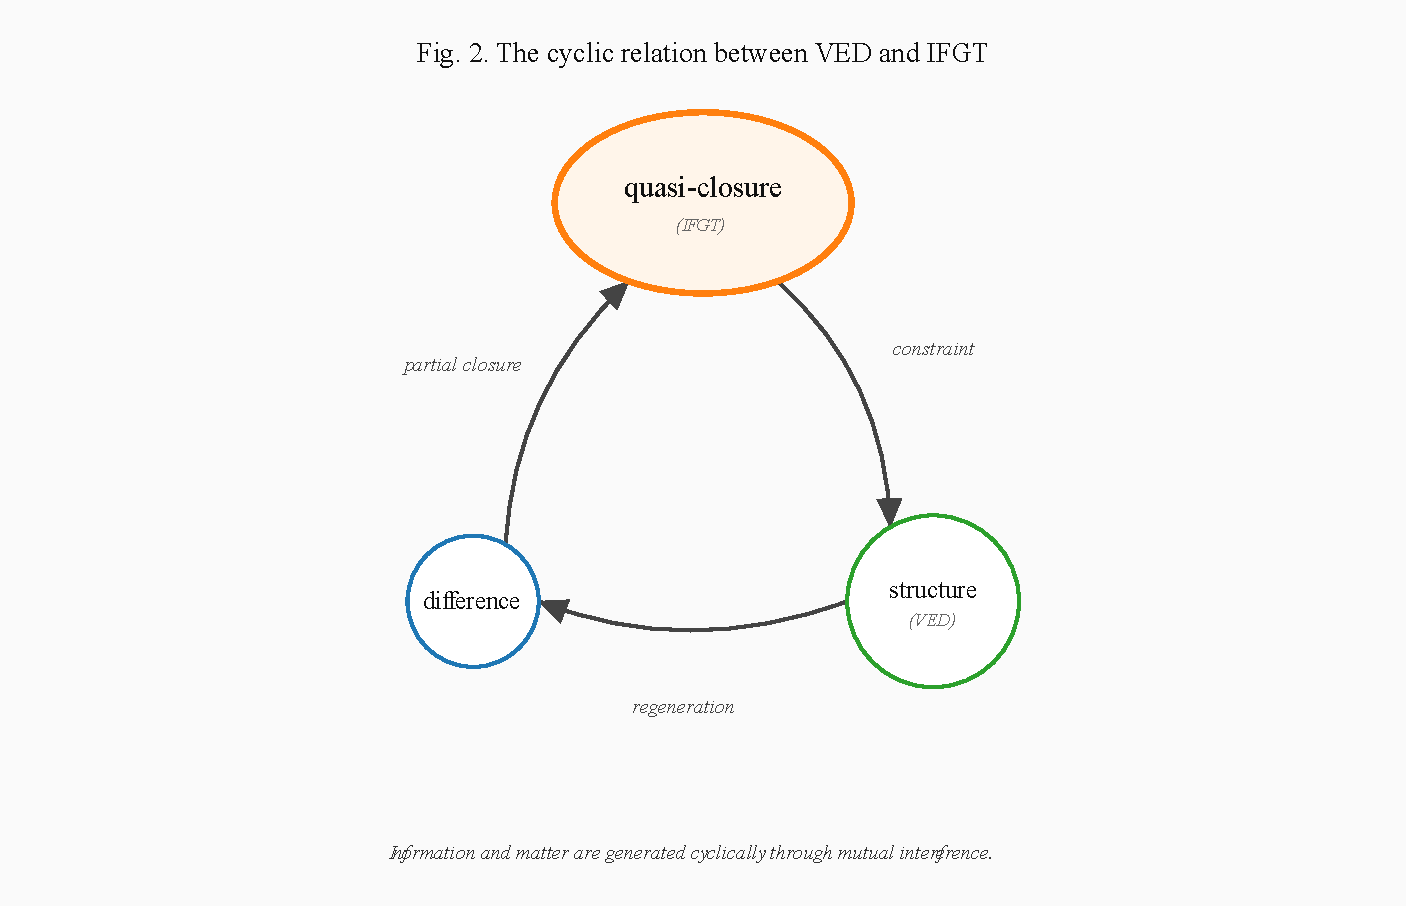
\includegraphics[width=0.80\textwidth]{figures/fig2_cyclic_relation_en.pdf}
  \caption{The cyclic relation between VED and IFGT. Information and matter are generated cyclically through mutual interference. The quasi-closure is positioned as the central mediating node.}
  \label{fig:cyclic_relation}
\end{figure}

This cycle is particularly prominent in the nervous systems of organisms, the memory of computers, and the internal states of transformer models, all of which are concrete examples of quasi-closures in which traces of difference are retained and subsequent flows are biased. This paper does not address these specific implementations but aims to describe the general structure underlying them.
